\section{Potential participants}
\label{sec:part}

\begin{wrapfigure}{!h}{3.2in}
  \vspace{-0.5cm}
  \centering 
  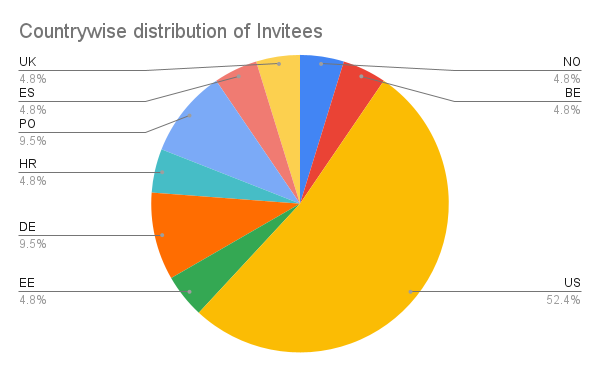
\includegraphics[scale=0.4]{fig/country.png}
  \caption{Country-wise break up of possible participant pool for \sympe.}
  \label{fig:country}
\end{wrapfigure}

We have shortlisted the following individuals as potential
participants in \sympe. We expect to prune this list down markedly to
the numbers we believe ($\sim 30$) which will make the symposium
viable to achieve the goals we have set out for it. It shows a broad
dispersion of disciplines, relevant to ocean observation, gender and
geography. Given the constraints of the symposium, including it being
held while there is substantial uncertainty in how the pandemic
situation will evolve, we believe it would be in the best interests to
narrow the participation to residents of the Americas and Europe. This
is reflected in the detail in Table \ref{tab:part} and is a starting
point to pull together the actual participants.


\begin{table}[H]
  \footnotesize{
\begin{tabular}{|p{3.5cm}|p{0.7cm}|p{4.0cm}|p{0.5cm}|p{6.0cm}|}
% {lllll}
  \rowcolor{Gray}
  \bfseries Name& \bfseries M/F&\bfseries Institution & \bfseries Country& \bfseries Specialization\\
  \ic{Aida Alvera Az\'{a}rate}    & F   & Univ. of Leige                        & BE       & Remote Sensing, modeling                        \\
  \hline
  \ic{Jo Eidsvik}               & M   & NTNU                                  & NO       & Statistical Sampling                            \\
  \hline
  \ic{Kanna Rajan}              & M   & SIFT LLC/Univ. of Porto            & US       & AI, Autonomous systems           \\
  \hline
  Maarja Krusma            & F   & Tallinn Inst. of Tech                 & EE  & Sensors/robotics                                \\
  \hline
  \ic{Ralf Bachmeyer}           & M   & Univ. of Bremen                       & DE       & Marine robotics, deep sea                       \\
  \hline
  \ic{Yogi Girdhar}             & M   & WHOI                                  & US       & Marine robotics + ML                            \\
  \hline
  \ic{Ajit Subramaniam}         & M   & Columbia Univ.                        & US       & Bio-optics, Oceanography                        \\
  \hline
  \ic{Pere Ridao}               & M   & Univ. of Girona& ES       & Grasping, robotics and control                            \\
  \hline
  \ic{Oliver Zelinsky}          & M   & Univ. of Oldernburg                   & DE       & Instrumentation, sensors                        \\
  \hline
  \ic{Peter Girguis}            & M   & Harvard                               & US       & Genomics, micro-biology                         \\
  \hline
  \ic{Shubha Satyendernath}     & F   & Plymouth Marine Labs                  & UK       & Remote Sensing, Ocean Color                     \\
  \hline
  \ic{Maha Haji}                & F   & Cornell Univ.                              & US       & Design optimization, Systems Engineering                   \\
  \hline
  Victoria Orphan          & F   & CalTech                               & US       & Microbial Ecology                               \\
  \hline
  \ic{Catarina Magahlaes}      & F   & CIIMAR, Univ. of Porto                & PO       & Biological Oceanography                         \\
  \hline
  Rick Stumpf              & M   & NOAA                                  & US       & HABs, Ocean Optics                              \\
  \hline
  \ic{Jo\~ao Vitorino}            & M   & Inst. Hidrografico                    & PO       & Physical Oceanography, modeling                    \\
  \hline
  \ic{Melissa Omand}            & F   & Univ. of Rhode Island                 & US       & Physical Oceanography                              \\
  \hline
  Chris Roman              & M   & Univ. of Rhode Island                 & US       & Sensors, instrumentation                        \\
  \hline
  Julien Brajard           & M   & Sorbonne / Nansen centre              & FR       & Data assimilation, machine learning             \\
  \hline
  \ic{Annalisa Bracco}          & F   & Georgia Tech                          & US       & Ocean physics, meso-scale dynamics              \\
  \hline
  Marta Chantal Ribeiro    & F   & UN \& Univ. of Porto                  & PO       & Law of the Sea                                  \\
  \hline
  \ic{Geoff Hollinger}          & M   & Oregon State Univ                     & US       & Robotics, Swarms, Sampling                              \\
  \hline
  Chelle Gentemann         & F   & Farallon Institute                    & US       & Remote Sensing (SST), air-sea fluxes \\
  \hline
  \ic{Ivona Cetinic}            & F   & NASA Goddard                            & US       & Ocean colour, ocean biogeochemistry  \\
  \hline
  \ic{Matjaz Licer}             & M   & NIB                                   & SL & Physical oceanography, ML, modelling            \\
  \hline
  \ic{Bastien Queste}           & M   & U. Gothenburg                         & SE       & Oceanographer, AUVs\\                            
  \hline
  Allison Schaap           & F   & Nat. Oceanography Center              & UK       & Micro-fluidics, ocean biogeochemistry, lab-on-a-chip\\
  \hline
  \ic{Sophie Clayton}           & F   & Old Dominion University              & US       & Phytoplankton Ecology, Physical-Biological Interactions\\
  \hline
  \ic{Marina Levy}              & F   & L'OCEAN                              & FR       & Ocean physics, biogeochemistry, plankton and marine ecosystems\\
  \hline
  Nikola Miskovic          & M   & Univ. of Zagreb                       & HR  & Marine robotics                                 \\
  \hline
  \ic{Pierre Lermusiaux}        & M   & MIT & US       &Modeling, assimilation \& prediction\\
  \hline
  \ic{Jo\~ao Sousa}               & M   & Univ. of Porto
                                                      & PO       &
                                                                   Control Systems + Marine robotics                      \\
  \hline
\end{tabular}
}
\caption{Potential invitee list (including organizers) to down-select
  from, for the \sympe. Names in \ic{red} have already confirmed their
  attendance.}
  \label{tab:part}
\end{table}

